\subsection{PickScore for W\"urstchen}
In their experiments, Pernias et al.~\cite{pernias2024wrstchen} are able to show
that their method yields a significant upgrade in computational costs and in
training time, which sits at a $8\times$ reduction compared to Stable Diffusion
2.1~\cite{rombach2023sd_2_1}. Another goal of the paper is to keep the level of
image complexity. In order to compare the level of complexity to other models,
Pernias et al. picked several evaluation methods. They used the
Fr\'echet Inception Distance~\cite{heusel2018ganstrainedtimescaleupdate} (see
Section~\ref{sec:experiments:stabel_diffusion:selction_of_fid}), the Inception
Score~\cite{ding2021cogviewmasteringtexttoimagegeneration}, and the human preference imitating
PickScore. Furthermore, they conducted a study with human participants. All were
given a text-prompt and the images of W\"urstchen and another model to compare.
In their experiments Pernias et al. found that W\"urstchen is capable to keep up or
even succeed over models of the same dimensions. While working with W\"urstchen
we found it to perform worse than presented by the authors. Thus, we
state our hypothesis that \textbf{W\"urstchen performs worse in the context of
    automated evaluation of human perception compared to the results of Pernias et al.}. Therefore, we
conduct experiments of the PickScore~\cite{kirstain2023pickapic} to
prove the correctness of our own suspicion. In this section, we first describe
the workings of PickScore, then we present the setup of our experiments and
after demonstrating our results we provide a discussion.

\subsubsection{Pick-a-Pic and PickScore}
\label{sec:wuerstchen:PickScore}
To imitate human users, language models have recently been trained to replicate
their behavior. For text-to-image models, Kirstain et
al.~\cite{kirstain2023pickapic} saw a gap for datasets and models that
indicate human preference. Thus, Kirstain et al. introduce the dataset
Pick-a-Pic which consists of data points that each have a prompt, two images which
were generated using this prompt, and the respective user preference. For
collecting the data, the authors constructed the Pick-a-Pic Web App that enables
its users to enter text-prompts. From these prompts, different model such as
Stable Diffusion 2.1~\cite{rombach2023sd_2_1}, Dreamlike Photoreal 2.0~\cite{dreamlike_art2024} and
Stable Diffusion XL~\cite{podell2024sdxl}. Two of these images are then
presented, and the user decides which image fits better to the prompt. The
not-preferred image is then replaced by a new image for the user to choose and so on. Kirstain et al.
mention that their application was used by intrinsically-motivated users who
they argue to yield better results than paid annotators as these users have
knowledge on how to shape a prompt in order to get the hoped result. The authors
add a recommendation for researchers to train their model on the Pick-a-Pic
dataset, because its prompts ``better represent what humans want to generate
than mundane captions, such as those found in MS-COCO''~\cite{kirstain2023pickapic}.

After establishing a rich dataset with a wide variety of prompts showing the
preference of users, Kirstain et al. created PickScore~\cite{kirstain2023pickapic}
to predict user preference. This model is based on the CLIP architecture. Thus,
it encodes a prompt $x$ and an image $y$ in form of $d$-dimensional
vector utilizing transformers. It takes the inner-product of these vectors to compute the scoring function
$s(x, y)$. PickScore employs $s(x, y)$ on two different images $y_1, y_2$ which
are both inherent to the prompt $x$. Additionally, the preference distribution
vector $p$ is available for the data triplet. Let $i$ be the index of the image
$y_i$, then the predicted preference distribution vector,
\begin{equation*}
    \hat{p}_i = \frac{\exp s(x, y_i)}{\sum_{j=1}^{2}\exp s(x, y_j)},
\end{equation*}
is calculated using the softmax-normalization. The model minimizes the
Kullback-Leibler Divergence~\cite{kullback1951OnInformationandSufficiency} during training to compute its predicted preference,
\begin{equation*}
    L_{pref} = \sum_{i=1}^{2} p_i (\log p_i - \log\hat{p}_i).
\end{equation*}
This training objective, is inspired
by the training objective of the InstructGPT reword model
objective~\cite{Ouyang2024InstructGPT}. In their experiments, Kirstain et al.
find that their method outperforms other competitors and even human experts.

\subsubsection{Experiment Description}
In this section, we demonstrate the setup of our experiment to confirm our
hypothesis stated above. To achieve this we re-do the PickScore
experiments conducted by Pernias et al., which they set as their primary
automated metric. Additionally, PickScore imitates human preference as we
describe in the preceding section which fits to the task of confirming our
suspicion. In our experiment, we only compare Stable Diffusion
2.1~\cite{rombach2023sd_2_1}, as its performance is the closest to W\"urstchen
among the worse-performing models in terms of PickScore, according to the
authors.

Concerning the prompts for image generation, we chose three different datasets.
First, we chose MSCOCO with localized narratives~\cite{PontTuset2020LocalizedNarratives}.
This dataset contains 5000 captions which are highly detailed and multimodal.
Secondly, we utilize Parti Prompts~\cite{yu2022scalingautoregressivemodelscontentrich}
containing 1633 prompts. These captions are highly diverse ranging from
not-detailed to very detailed. Pernias et al. mention that this dataset reflects
the use-case that they intend for their model. In contrast to MSCOCO with
localized narratives and Parti Prompts the last dataset was not employed by the
authors of W\"urstchen. For this, we follow the recommendation of Kirstain et
al.~\cite{kirstain2023pickapic} and choose Pick-a-Pic as our last dataset. The
validation set includes 500 prompts, which all were created by people who are
``are actual text-to-image users''\cite{kirstain2023pickapic}.

In order to show the stability of the PickScore results, we conduct five
iteration for each prompt, which results in five images for the respective
prompt and each model. For one iteration, we average across all preference
values and take the mean over all five iterations for a model.

\subsubsection{Results and Discussion}
\begin{table}[t]
    \caption{This table presents the mean results of Pernias et
        al.\cite{pernias2024wrstchen}, and mean and standard deviation of our
        experiments. We provide the results for the MSCOCO localized narratives
        (MSCOCO LN) dataset, the Parti Prompt dataset and the Pick-a-Pic
        dataset. Each value shows the mean portion of prompts that yield images
        of W\"urstchen which are preferred by the PickScore model over the
        images of Stabel Diffusion 2.1.}
    \label{tab:wuerstchen:results}
    \centering
    \begin{tabular}{lccccccc}
        \toprule
        \textbf{W\"urstchen}                     & \textbf{MSCOCO LN}    & \phantom{0} & \textbf{Parti Prompt} & \phantom{0} & \textbf{Pick-a-Pic}   \\
        \midrule
        Pernias et al.\cite{pernias2024wrstchen} & 70.0\%                & \phantom{0} & 74.6\%                & \phantom{0} & -                     \\
        Our Results                              & 65.8\%{\tiny$\pm1.0$} & \phantom{0} & 67.8\%{\tiny$\pm0.9$} & \phantom{0} & 73.4\%{\tiny$\pm0.8$} \\
        \bottomrule
    \end{tabular}
\end{table}
In the preceding section, we present the setup of our experiments. In this
section, we demonstrate our results and discuss them.
Table~\ref{tab:wuerstchen:results} shows the results for each dataset together
with the results of Pernias et al.~\cite{pernias2024wrstchen}. Furthermore,
Table~\ref{tab:wuerstchen:example} provides two examples of prompt from each
dataset and the respective images that we generated during the execution of our
experiments. The results show a decrease in the PickScore (see
Section~\ref{sec:wuerstchen:PickScore}) for both datasets that were included in
the original paper, of MSCOCO localized
narratives~\cite{PontTuset2020LocalizedNarratives} (MSCOCO LN) and Parti
Prompts~\cite{yu2022scalingautoregressivemodelscontentrich}.
Pick-a-Pic~\cite{kirstain2023pickapic} prompts exhibit a high PickScore
preference towards W\"urstchen. For all three datasets, the standard deviation
keeps at around 1\%.

Our results simultaneously confirm our hypothesis and stay according to the
conclusion of the W\"urstchen authors. Our hypothesis build on the results
from Pernias et al. not reflecting our own perception of the images from the
model. This is proven by the decrease of the human preference imitating
PickScore. Meanwhile, the preferences stay high enough to show that W\"urstchen can
compete with the image quality of Stable Diffusion 2.1 while decreasing the
training time. Finally, the PickScore on the Pick-a-Pic dataset shows that
W\"urstchen produces images with a higher quality concerning prompts from
real world cases.

\begin{table}[hbp]
    \centering
    \addtolength{\leftskip}{-0.65cm}
    \caption{Exemplary visualization of the images generated during our
        experiments. The first row provides the instances of the prompts from the
        respective datasets. In the second and third row we provide the images
        generated by Stable Diffusion 2.1~\cite{rombach2023sd_2_1} and
        W\"urstchen~\cite{pernias2024wrstchen} for these prompts respectively.}
    \label{tab:wuerstchen:example}
    \scalebox{0.7}{
        \begin{tabular}{ccccccccc}
                                                                                                    & \multicolumn{2}{c}{\textbf{MSCOCO LN}}                                                       & \phantom{0}                                                                                    & \multicolumn{2}{c}{\textbf{Parti Prompt}} & \phantom{0}                                                                              & \multicolumn{2}{c}{\textbf{Pick-a-Pic}}                                                                                                                                                                                                                                                      \\
            \cmidrule{2-3}\cmidrule{5-6}\cmidrule{8-9}                                                                                                                                                                                                                                                                                                                                                                                                                                                                                                                                                                                                                                                                                    \\
            \rotatebox[origin=c]{90}{prompts}                                                       & \makecell{(...) a person who                                                                                                                                                                                                                                                                                                                                                                                                                                                                                                                                                                                                        \\is standing and\\holding baseball\\bat (...) ground\\and spectators\\are watching (...)} &\makecell{In the picture\\we can see a\\bun with pink\\color food item.}& \phantom{0}& bond & \makecell{a pickup truck\\kicking up dust\\on a back road} & \phantom{0} & \makecell{Apocalyptic scenes\\of a meteor\\storm over\\a volcano.} & \makecell{A girl playing\\a violin, in the\\style of your\\lie in april} \\
            \raisebox{1.45\height}{\rotatebox[origin=c]{90}{SD 2.1~\cite{rombach2023sd_2_1}}}       & 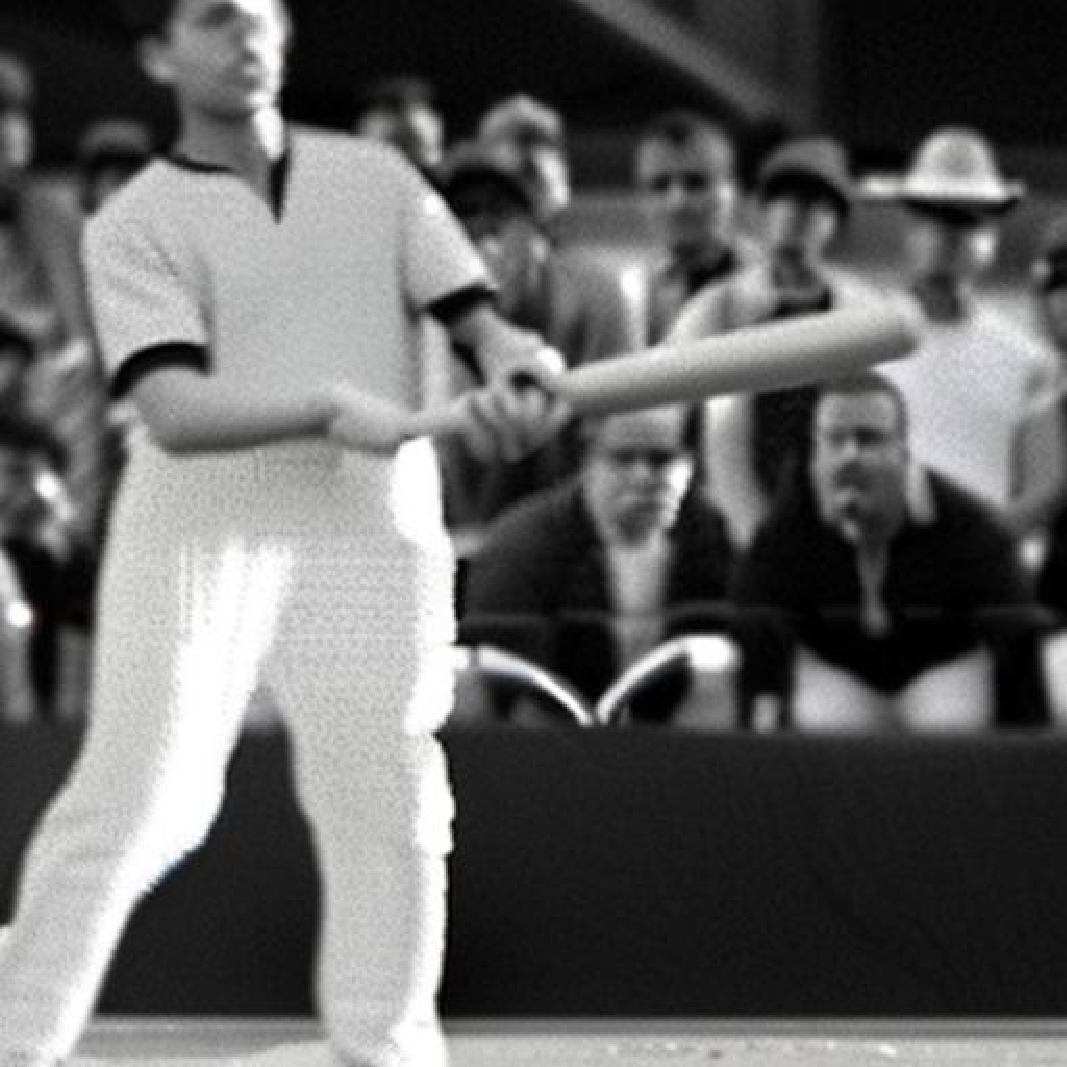
\includegraphics[width=0.2\textwidth]{assets/Model.SD2_1_Datasets.NARRATIVE_MSCOCO.pdf}      & 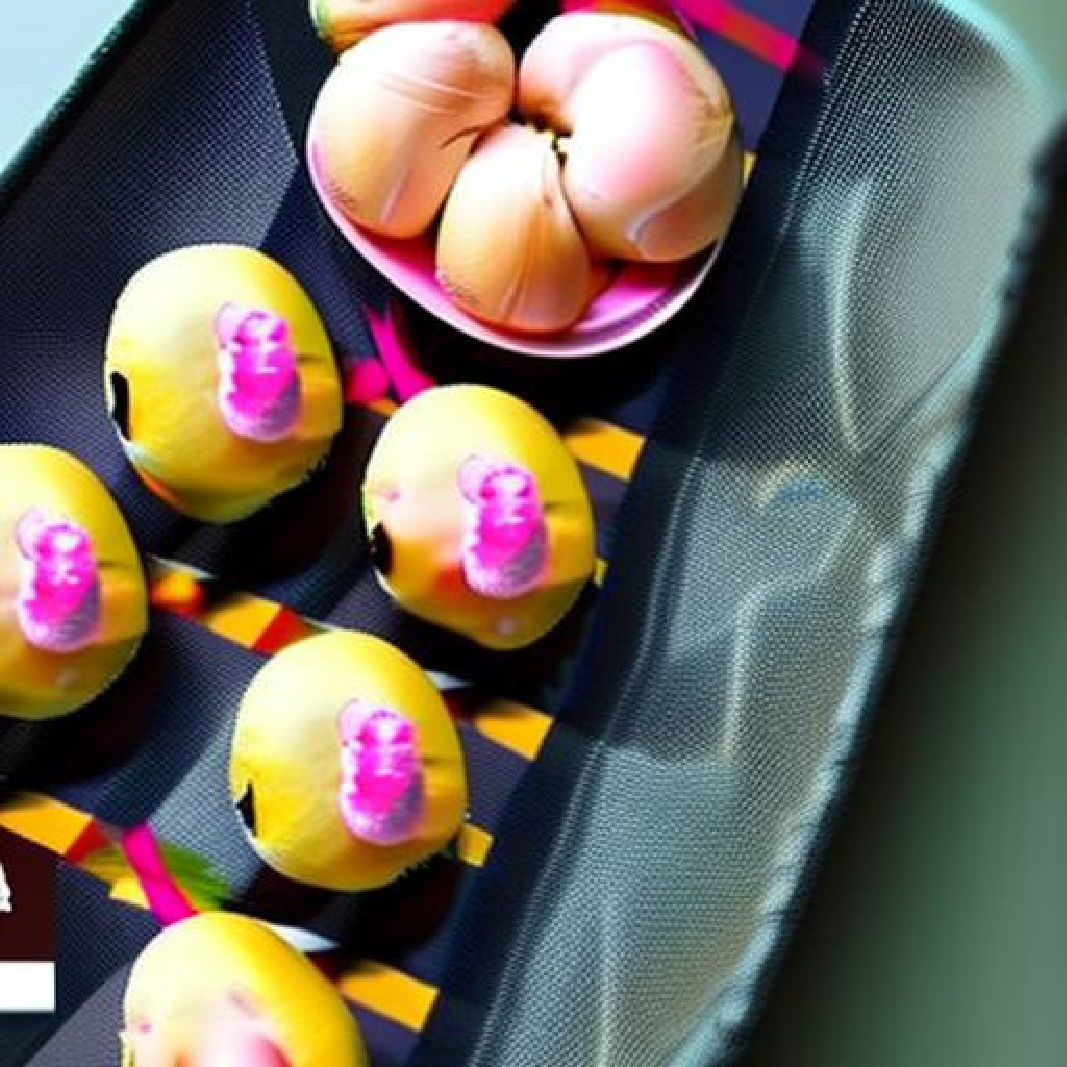
\includegraphics[width=0.2\textwidth]{assets/Model.SD2_1_Datasets.NARRATIVE_MSCOCO_1.pdf}      & \phantom{0}                               & 
\includegraphics[width=0.2\textwidth]{assets/Model.SD2_1_Datasets.PARTI_PROMPT.pdf}      & 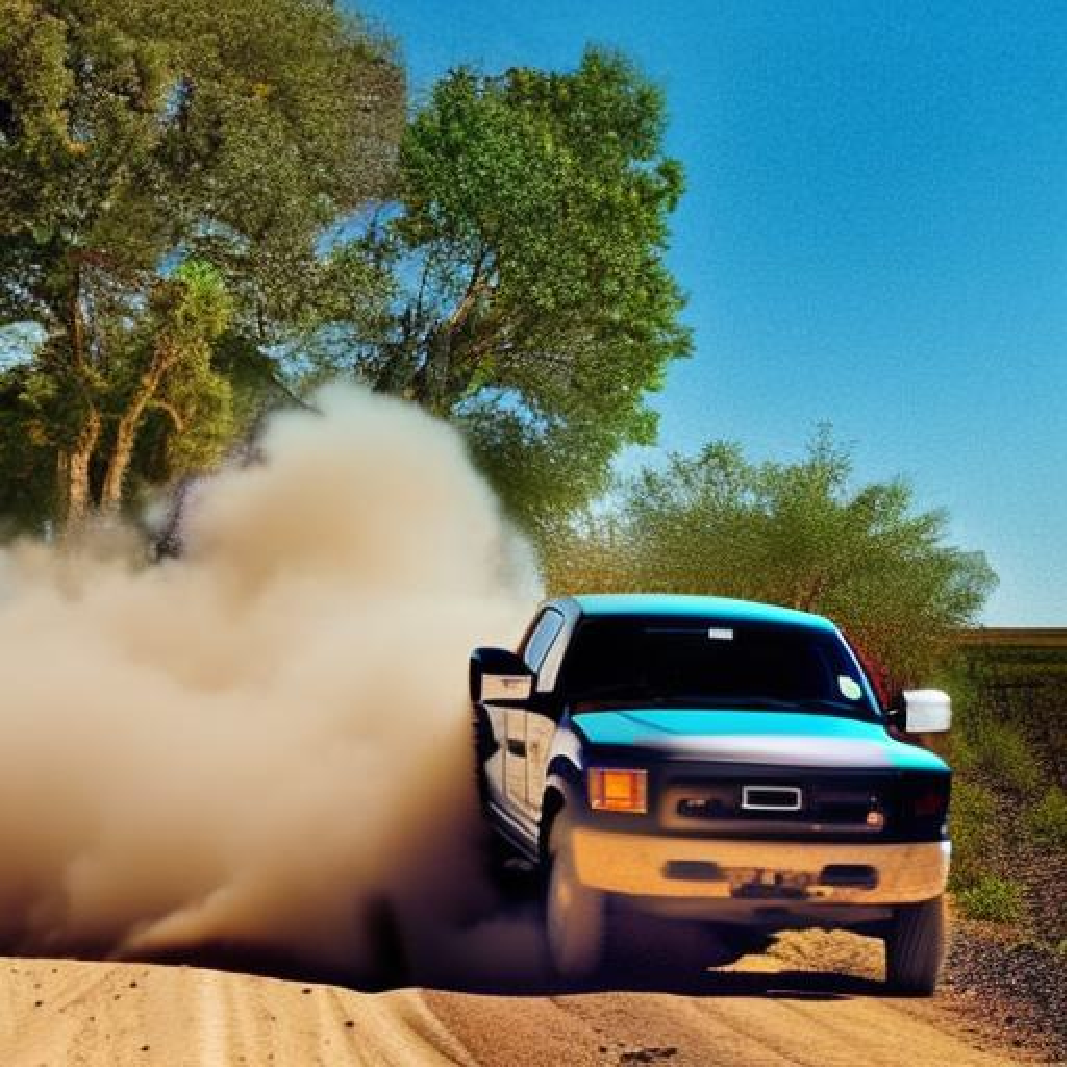
\includegraphics[width=0.2\textwidth]{assets/Model.SD2_1_Datasets.PARTI_PROMPT_1.pdf}      & \phantom{0} & 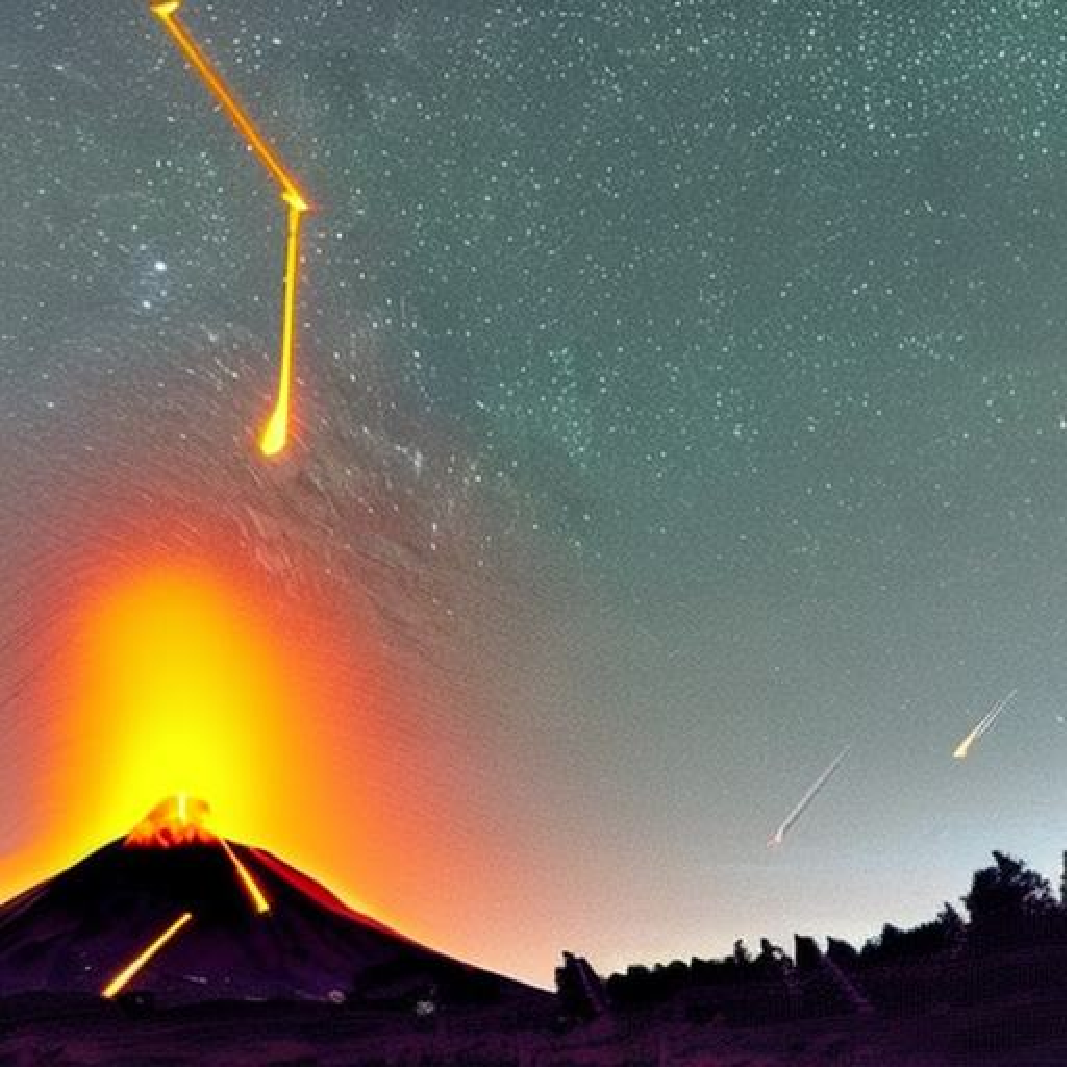
\includegraphics[width=0.2\textwidth]{assets/Model.SD2_1_Datasets.Pick_A_Pic.pdf}      & 
\includegraphics[width=0.2\textwidth]{assets/Model.SD2_1_Datasets.Pick_A_Pic_1.pdf}      \\
            \raisebox{1.2\height}{\rotatebox[origin=c]{90}{W\"urstchen~\cite{pernias2024wrstchen}}} & 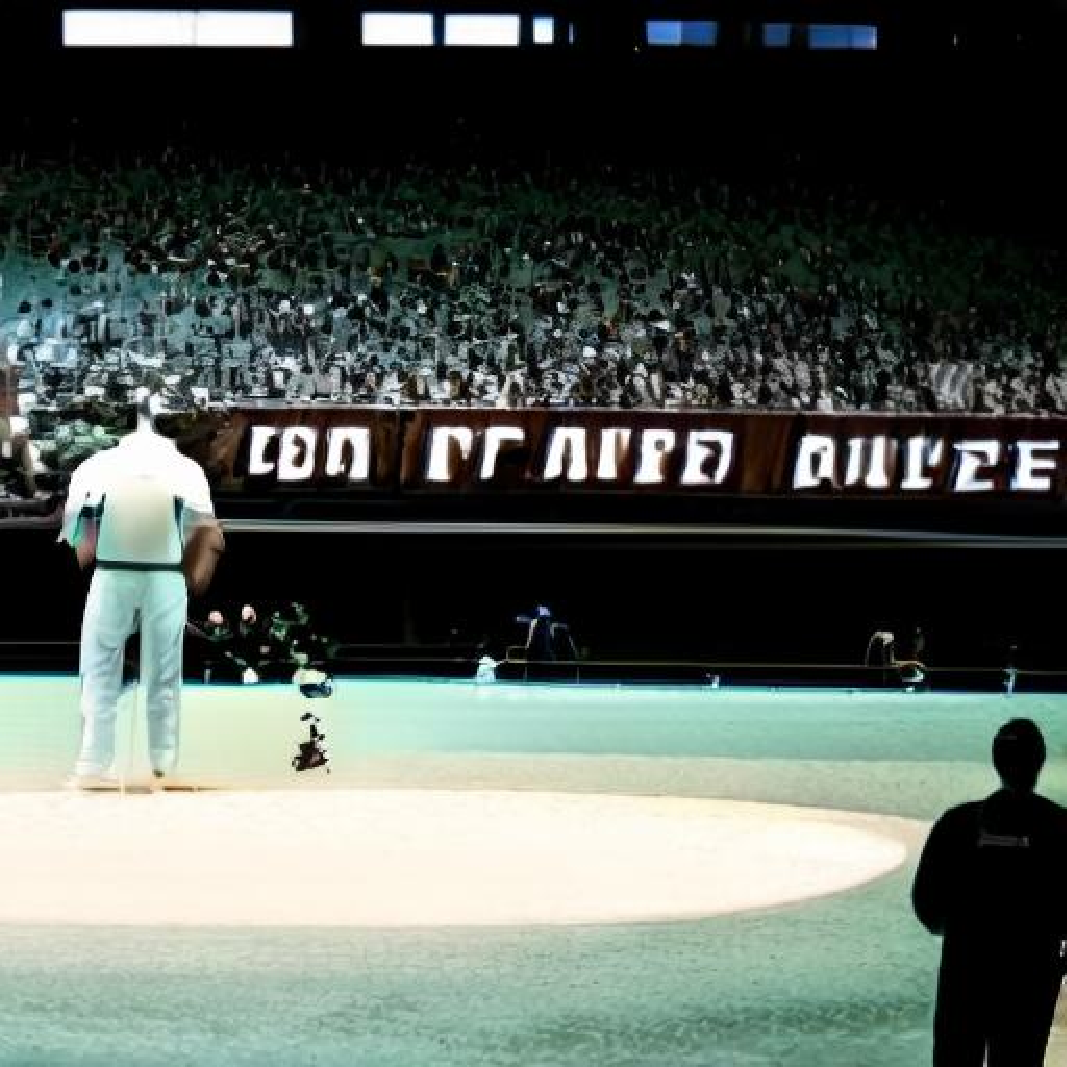
\includegraphics[width=0.2\textwidth]{assets/Model.Wuerstchen_Datasets.NARRATIVE_MSCOCO.pdf} & 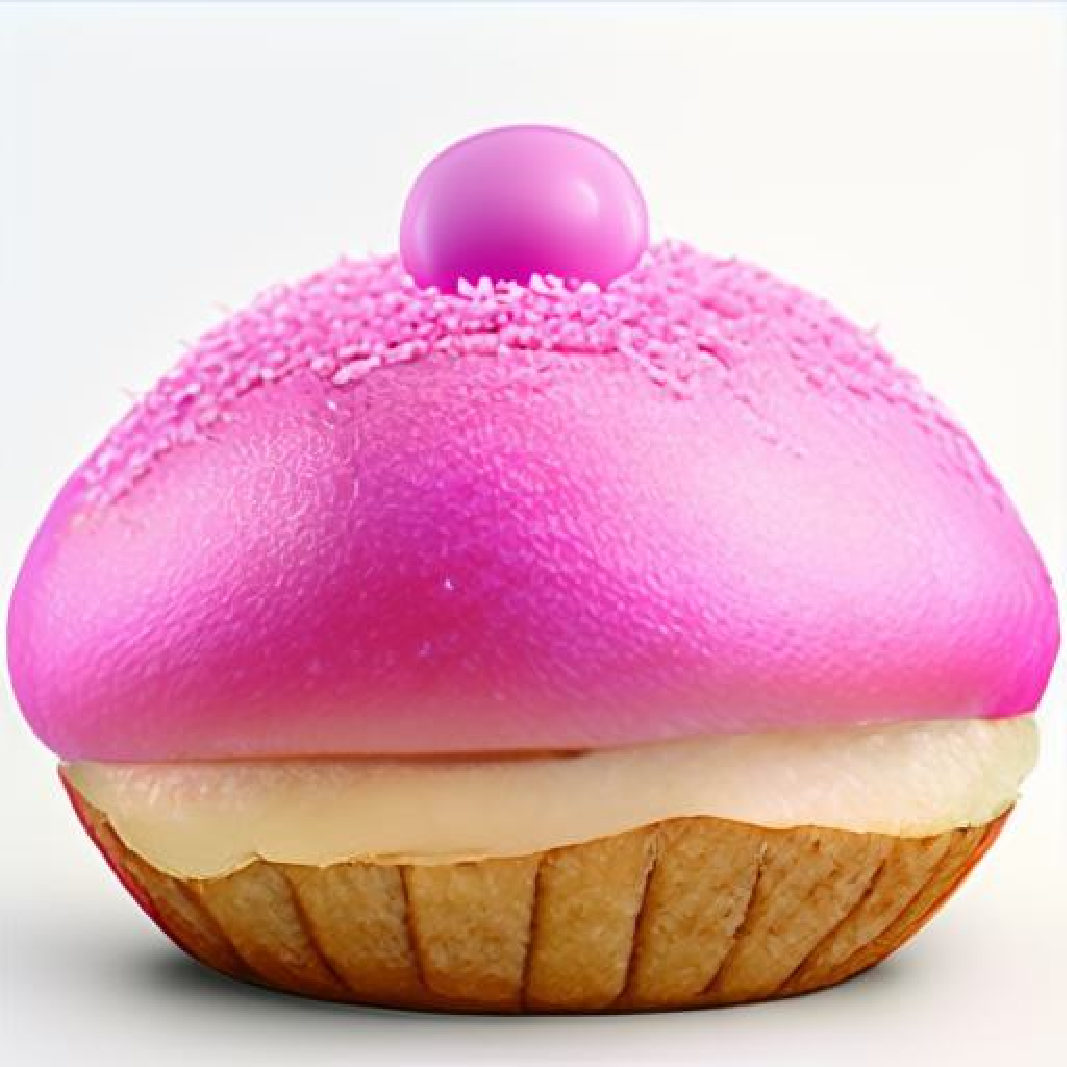
\includegraphics[width=0.2\textwidth]{assets/Model.Wuerstchen_Datasets.NARRATIVE_MSCOCO_1.pdf} & \phantom{0}                               & 
\includegraphics[width=0.2\textwidth]{assets/Model.Wuerstchen_Datasets.PARTI_PROMPT.pdf} & 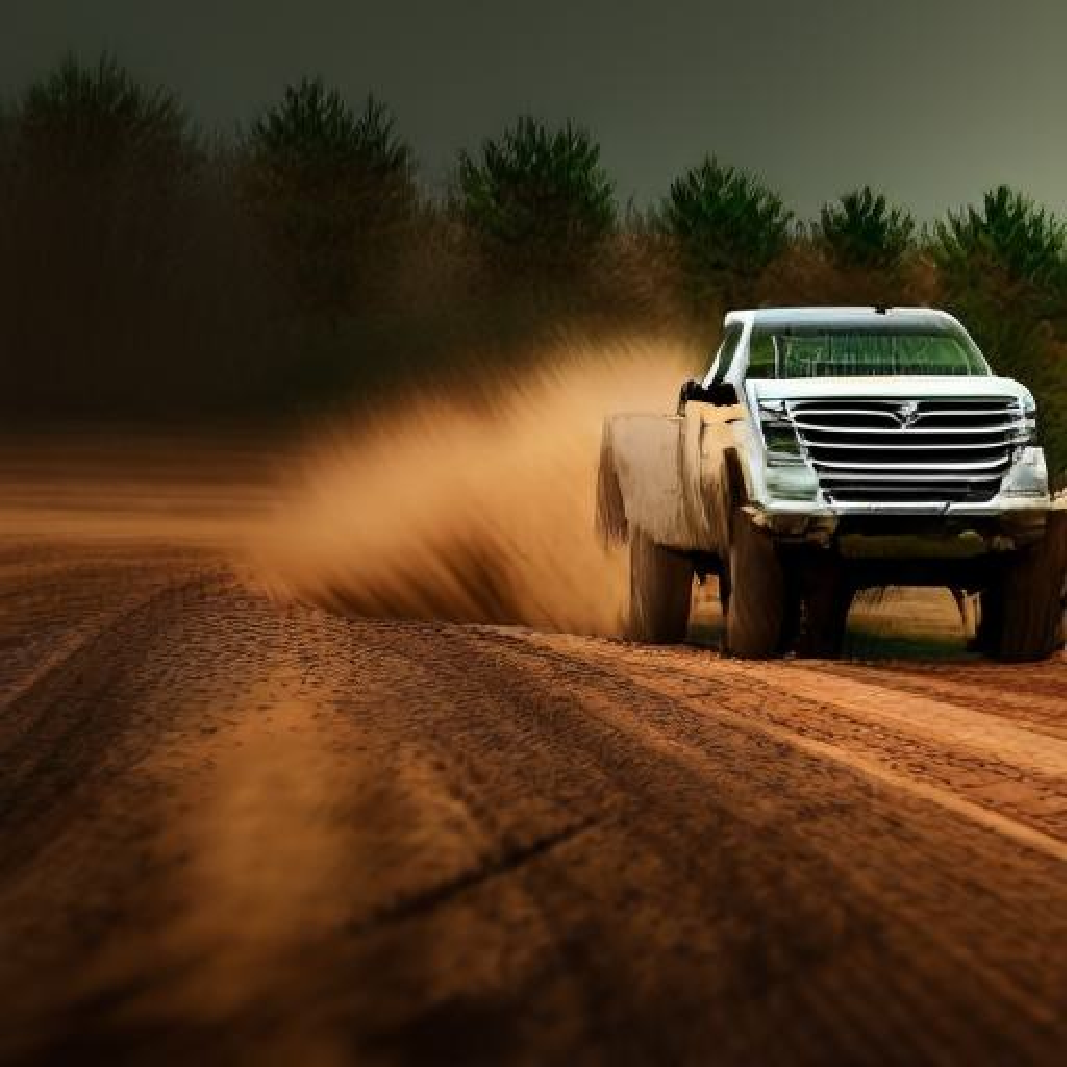
\includegraphics[width=0.2\textwidth]{assets/Model.Wuerstchen_Datasets.PARTI_PROMPT_1.pdf} & \phantom{0} & 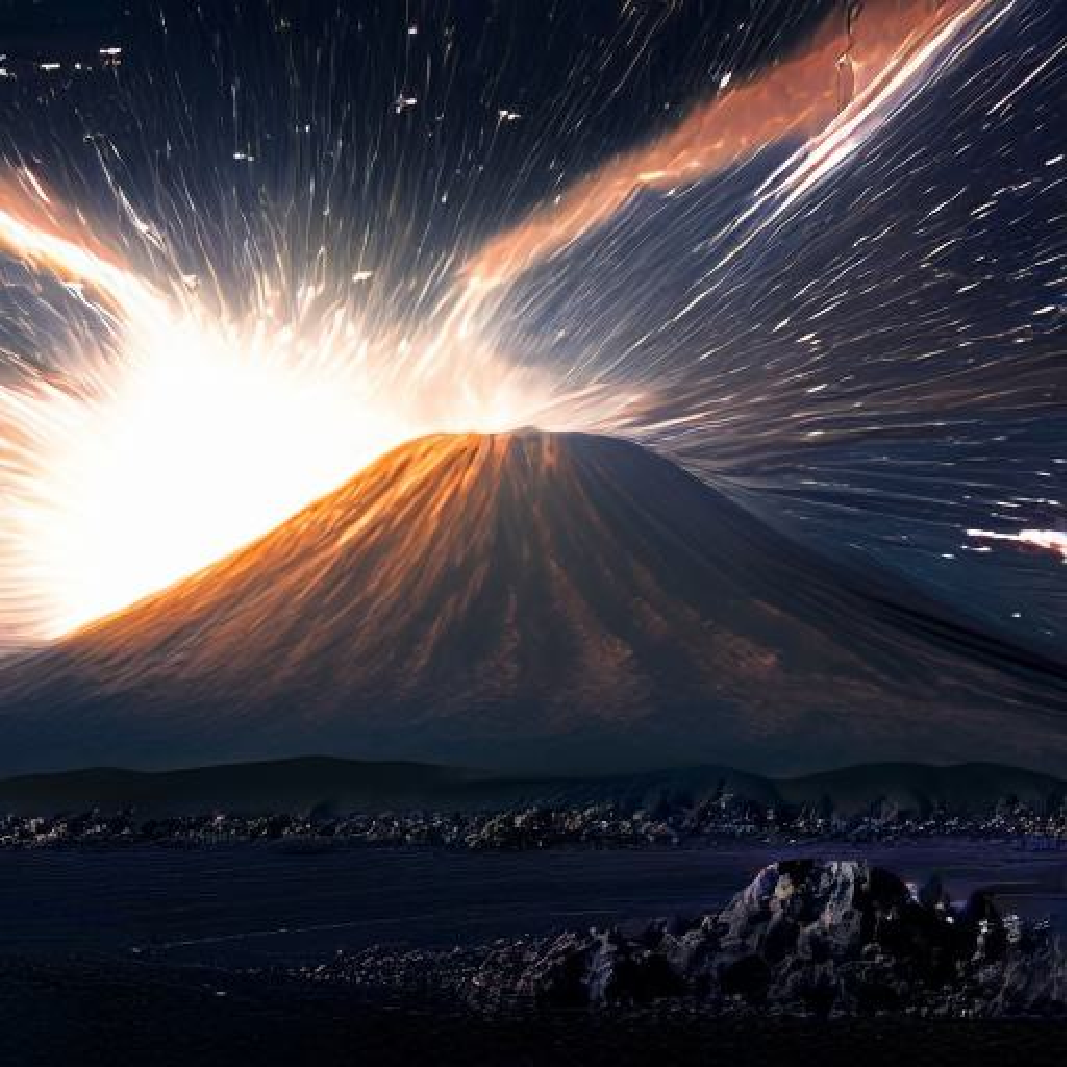
\includegraphics[width=0.2\textwidth]{assets/Model.Wuerstchen_Datasets.Pick_A_Pic.pdf} & 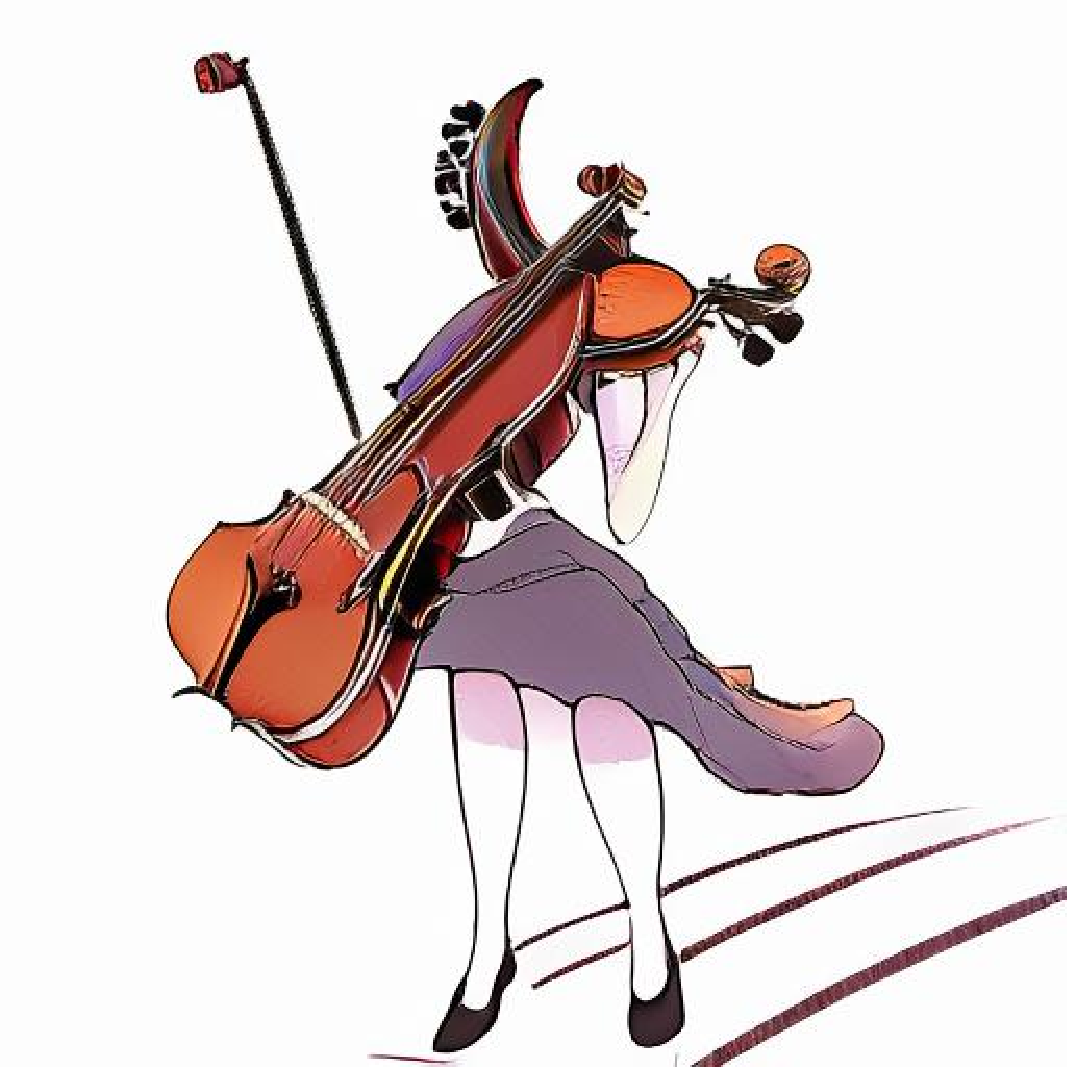
\includegraphics[width=0.2\textwidth]{assets/Model.Wuerstchen_Datasets.Pick_A_Pic_1.pdf} \\
        \end{tabular}
    }
\end{table}
